	\chapter{Экспериментальный раздел}
\label{cha:research}
    В данном разделе будут проведены эксперименты 
    для сравнительного анализа трёх алгоритмов по затрачиваемому процессорному 
    времени в зависимости от индекса слова в словаре.

    \section{Сравнительный анализ на основе замеров времени работы алгоритмов}
        В рамках данного проекта были проведёны эксперименты
        по замеру времени работы алгоритмов поиска слова в словаре:
        \begin{enumerate}
            \item полным перебором (график \ref{graph:test:brute-force});
            \item двоичным поиском (график \ref{graph:test:binary});
            \item поиском по сегментам (график \ref{graph:test:segment}).
        \end{enumerate}

        \begin{figure}[h!]
            \centering
                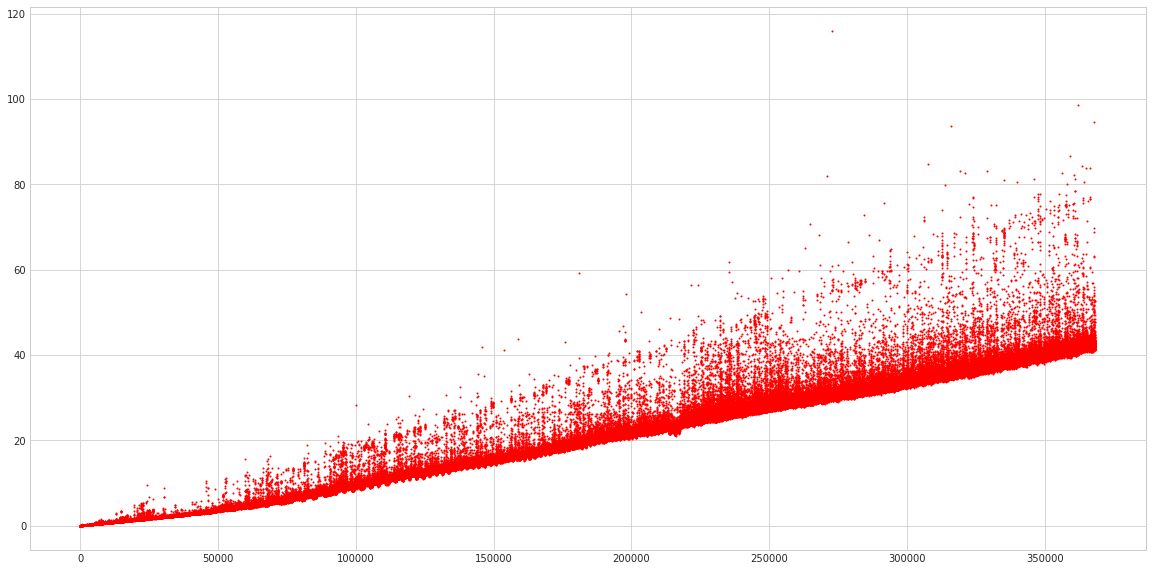
\includegraphics[height=0.74\textheight]{BruteForce.png}
                \caption{Время поиска слова в словаре полным перебором}
                \label{graph:test:brute-force}
        \end{figure}


        
        \begin{figure}[h!]
            \centering
                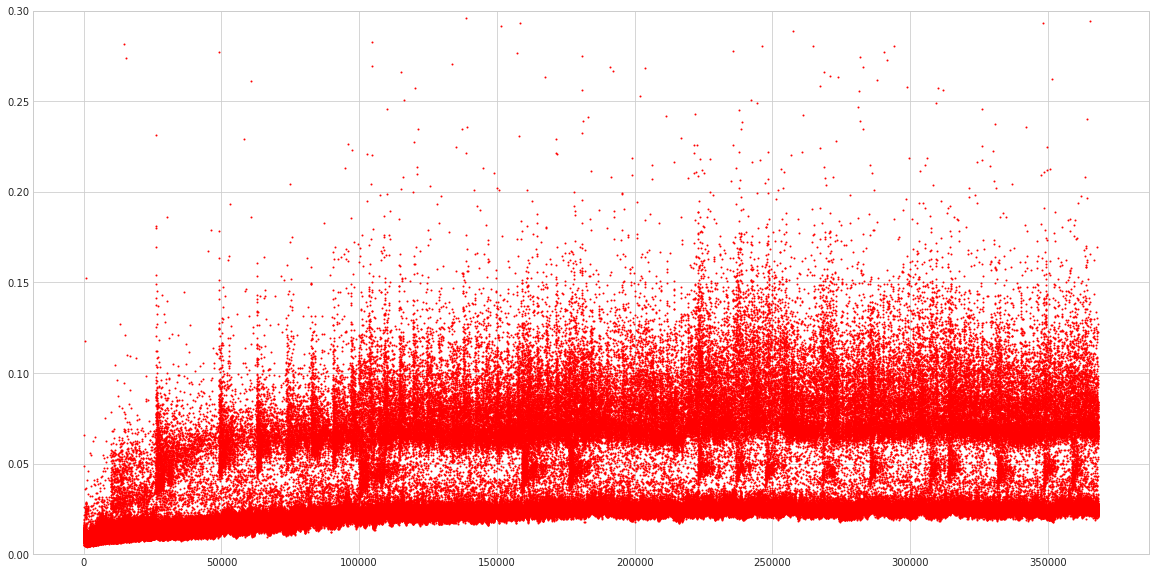
\includegraphics[height=0.74\textheight]{BinarySearch.png}
                \caption{Время двоичного поиска слова в словаре}
                \label{graph:test:binary}
        \end{figure}

        \begin{figure}[h!]
            \centering
                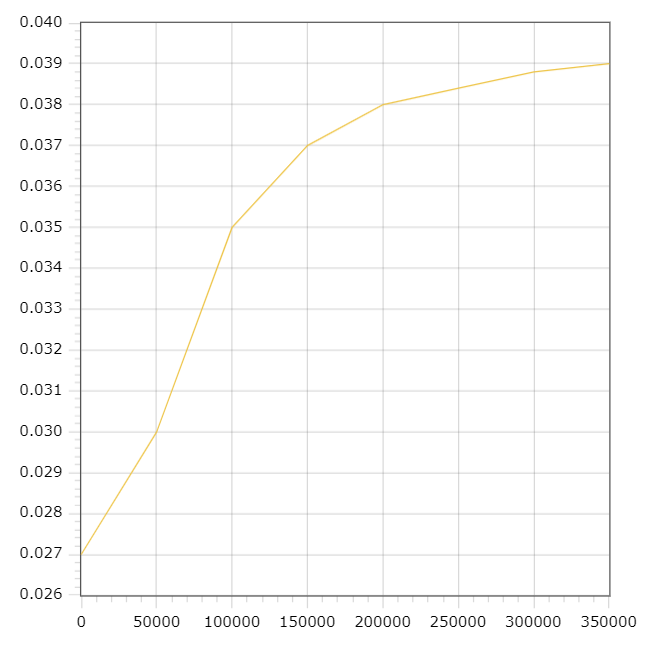
\includegraphics[height=0.74\textheight]{SegmentSearch.png}
                \caption{Время поиска слова по сегментам в словаре}
                \label{graph:test:segment}
        \end{figure}

    \section{Статистический анализ замеров}
        По графику \ref{graph:test:brute-force} видно, 
        что время поиска линейно.
        В худших случаях алгоритму требуется 42 секунды 
        на поиск последего слова из набора или же несуществующего. 

        В среднем бинарному поиску требуется примерно ~0.040 секунд.
        В то время как алгоритму поиска по сегментам
        необходимо ~0.037. 

    \section{Вывод}
        В ходе экспериментов по замеру времени работы было установлено, что 
        самым эффективным и стабильным является поиск по сегментам.
        Самым долгим является алгоритм полного перебора.
        Его время возрастает каждый раз из-за того, 
        что слова находятся дальше в словаре, 
        а каждый раз поиск начинается с самого начала. 
        По графикам алгоритма бинарного поиска и поиска по сегментам 
        можно увидеть нормальное распределение времени поиска слова в словаре.
        на данных тестовых данных 

\newpage